\section{GE in an Endowment Economy}

\begin{frame}

\begin{center}
{\LARGE GE in an Endowment Economy}
\end{center}

\end{frame}

%------------------------------------------------
%------------------------------------------------

\begin{frame}{Simple consumption-savings problem of household}

We begin with an optimization of a price-taking household
\begin{itemize}
\item Utility is intertemporally separable
\item Period `felicity' function $U(c_{t}^{i})$
\item Household $i$ receives known endowment $\left\{ y_{t}^{i}\right\}_{t=0}^{\infty }$
\item Savings $\left\{ a_{t}^{i}\right\}_{t=0}^{\infty }$ earn known interest rate $\left\{ R_{t}=(1+r_{t})\right\} _{0}^{\infty }$
\item \textbf{No uncertainty (`DGE' for now)}
\item Household chooses savings and consumption
\end{itemize}

\vspace{2mm}
Ultimately, the problem of the household (or households) will be one part of the equilibrium
\begin{itemize}
\item	Will also eventually need firm optimality, market clearing and feasibilty conditions\ldots
\end{itemize}
\end{frame}

%------------------------------------------------
%------------------------------------------------

\begin{frame}{Household budget constraint}

Flow budget constraint (note timing of return on wealth in this model without uncertainty)
\begin{equation*}
a_{t+s+1}^{i}=R_{t+s}a_{t+s}^{i}+y_{t+s}^{i}-c_{t+s}^{i}\text{ for }\forall s\geq 0
\end{equation*}
Iterate forward
\begin{equation*}
\prod\limits_{t=0}^{T}R_{t}^{-1}a_{T+1}^{i}=a_{0}^{i}+\sum_{t=0}^{T}\left(\prod\limits_{s=0}^{t}R_{s}^{-1}\right) \left( y_{t}^{i}-c_{t}^{i}\right)
\end{equation*}
Present value budget constraint
\begin{equation*}
\frac{a_{T+1}^{i}}{\tilde{R}_{T}}=a_{0}^{i}+\sum\limits_{t=0}^{T}\frac{y_{t}^{i}-c_{t}^{i}}{\tilde{R}_{t}}
\end{equation*}
\begin{itemize}
\item[]	where $\tilde{R}_{t} \equiv R_{0}R_{1}R_{2}\ldots R_{t}$
\end{itemize}

\end{frame}

%------------------------------------------------
%------------------------------------------------

\begin{frame}{Household budget constraint}

Present value budget constraint
\begin{equation*}
\underbrace{\frac{a_{T+1}^{i}}{\tilde{R}_{T}} +\sum\limits_{t=0}^{T}\frac{c_{t}^{i}}{\tilde{R}_{t}}}_{Uses} = \underbrace{a_{0}^{i}+\sum\limits_{t=0}^{T}\frac{y_{t}^{i}}{\tilde{R}_{t}}}_{Sources}
\end{equation*}

You only get utility from $c_{t}$ sequence and suppose your `sources' are fixed
\begin{itemize}
\item	How to make PV of consumption $>$ than `sources', for $T<\infty$?
\item	Offset with negative $\frac{a_{T+1}^{i}}{\tilde{R}_{T}}$ (interpretation?)
\end{itemize}

Let $T \rightarrow \infty$, does this seem plausible?
\begin{itemize}
\item	Assuming $R_{t} > 1$ this is going to require \textit{explosive} debt
\item	Standard to rule that out
\item	$a_{T}$ can be negative in limit - it's only the PV that must be $\geq 0$
\end{itemize}

\end{frame}

%------------------------------------------------
%------------------------------------------------

\begin{frame}{Transversality condition (TVC)}

No \href{https://en.wikipedia.org/wiki/Ponzi_scheme}{Ponzi} condition to rule out explosive borrowing
	\begin{itemize}
	\item	PV of terminal saving `cannot' be strictly negative
	\item	No-one is going to give you a free lunch
	\end{itemize}
\begin{equation*}
\lim_{T\rightarrow \infty} \frac{a_{T+1}^{i}}{\tilde{R}_{T}}\geq 0
\end{equation*}

PV of terminal saving `won't' be $>0$ as would be individually suboptimal
	\begin{itemize}
	\item	Note this is a distinct issue from No Ponzi
	\item	Can weakly increase $c_{t}$ in all periods and strictly in at least one
	\item	\textit{Feasible} improvement contradicts optimality requirement
	\end{itemize}
\vspace{1.5mm}
Thus, condition will in fact hold with equality in equilibrium (TVC)
\begin{itemize}
\item	Present value BC $\Leftrightarrow$ PV of consumption $=$ PV of resources
\end{itemize}
\begin{equation*}
\sum\limits_{t=0}^{\infty }\frac{c_{t}^{i}}{\tilde{R}_{t}}=a_{0}^{i}+\sum\limits_{t=0}^{\infty }\frac{y_{t}^{i}}{\tilde{R}_{t}}
\end{equation*}

\end{frame}

%------------------------------------------------
%------------------------------------------------

\begin{frame}{Household problem}

\begin{gather*}
\underset{\{c_{t+s}^{i},a_{t+s+1}^{i}\}}{\max }\underset{s=0}{\overset{\infty }{\sum }}\beta ^{s}U(c_{t+s}^{i}) \\[0.3cm]
\text{s.t.} \\[0.3cm]
a_{t+s+1}^{i}=R_{t+s}a_{t+s}^{i}+y_{t+s}^{i}-c_{t+s}^{i}\text{ for }\forall s\geq 0 \\[0.5cm]
a_{t}^{i}\text{ given,}\\[0.3cm]
\underset{T\rightarrow \infty }{\lim }\frac{a_{T+1}^{i}}{\tilde{R}_{T}}\geq 0
\end{gather*}

\end{frame}

%------------------------------------------------
%------------------------------------------------

\begin{frame}{Solution Method \#1: Direct substitution}

Substitute for $c_{t+s}^{i}$ in utility function using flow budget constraint%
\begin{equation*}
\underset{\{a_{t+s+1}^{i}\}}{\max }\underset{s=0}{\overset{\infty }{\sum }}\beta ^{s}U(R_{t+s}a_{t+s}^{i}+y_{t+s}^{i}-a_{t+s+1}^{i})
\end{equation*}

First order condition with respect to $a_{t+1}^{i}$
\begin{equation*}
-U_{c^{i},t}+\beta U_{c^{i},t+1}R_{t+1}=0
\end{equation*}

Intertemporal \textcolor{red}{\textbf{Euler equation}} for consumption
\begin{equation*}
\beta R_{t+1}\frac{U_{c^{i},t+1}}{U_{c^{i},t}}-1=0
\end{equation*}

\end{frame}

%------------------------------------------------
%------------------------------------------------

\begin{frame}{Method \#2: Graphical}
Expand utility function
\begin{equation*}
\underset{s=0}{\overset{\infty }{\sum }}\beta^{s}U(c_{t+s}^{i})=U(c_{t}^{i})+\beta U(c_{t+1}^{i})+\ldots =\bar{U}
\end{equation*}
Total differentiation taking $\bar{U}$ and $c_{t+s}^{i}$ as given $\forall s\geq 2$ 
\begin{equation*}
\frac{dc_{t+1}^{i}}{dc_{t}^{i}}=-\frac{1}{\beta }\frac{U_{c^{i},t}}{%
U_{c^{i},t+1}}=\text{MRS}
\end{equation*}
Indifference curve in $(c_{t}^{i},c_{t+1}^{i})$ space
\begin{figure}
\centering
\label{fig:intertemp_c_icurve}
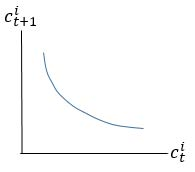
\includegraphics[width=0.3\textwidth]{Figures/intertemp_c_icurve.JPG}
\end{figure}
\end{frame}

%------------------------------------------------
%------------------------------------------------

\begin{frame}{Method \#2:\ Graphical}
Expand budget constraint
\begin{equation*}
a_{t+2}^{i}=R_{t+1}\left( R_{t}a_{t}^{i}+y_{t}^{i}-c_{t}^{i}\right)+y_{t+1}^{i}-c_{t+1}^{i}
\end{equation*}

Total differentiation taking $a_{t}^{i},a_{t+2}^{i},y_{t}^{i}$ and $y_{t+1}^{i}$ as given 
\begin{equation*}
\frac{dc_{t+1}^{i}}{dc_{t}^{i}}=-R_{t+1}=\text{MRT}
\end{equation*}

Budget constraint in $(c_{t}^{i},c_{t+1}^{i})$ space
\begin{figure}
\centering
\label{fig:intertemp_c_bconstraint}
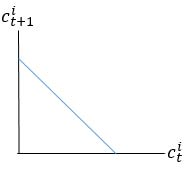
\includegraphics[width=0.3\textwidth]{Figures/intertemp_c_bconstraint.JPG}
\end{figure}
\end{frame}

%------------------------------------------------
%------------------------------------------------

\begin{frame}{Method \#2:\ Graphical}
Optimising household sets MRS=MRT 
\begin{equation*}
\beta R_{t+1}\frac{U_{c^{i},t+1}}{U_{c^{i},t}}-1=0
\end{equation*}
Optimality in $(c_{t}^{i},c_{t+1}^{i})$ space
\begin{figure}
\centering
\label{fig:intertemp_c_tangency}
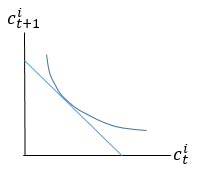
\includegraphics[width=0.3\textwidth]{Figures/intertemp_c_tangency.JPG}
\end{figure}
\end{frame}

%------------------------------------------------
%------------------------------------------------

\begin{frame}{Method \#3:\ Value function}
Value function (this is a very brief illustration of this advanced technique)
\begin{equation*}
V(a_{t}^{i})=\underset{a_{t+1}^{i}}{\max }\left[U(R_{t}a_{t}^{i}+y_{t}^{i}-a_{t+1}^{i})+\beta V(a_{t+1}^{i})\right]
\end{equation*}
First order condition still involves $V$, which is not yet explicitly, defined
\begin{equation*}
U_{c^{i},t}=\beta V^{\prime }(a_{t+1}^{i})
\end{equation*}
Differentiate $V(a_{t}^{i})$ w.r.t. $a_{t}^{i}$ (an \href{https://en.wikipedia.org/wiki/Envelope_theorem}{envelope condition} is being used) here)
\begin{equation*}
V^{\prime }(a_{t}^{i})=U_{c^{i},t}R_{t}
\end{equation*}
Then just roll forward one period and substitute for $V^{\prime }(a_{t+1}^{i})$
\begin{equation*}
\beta R_{t+1}\frac{U_{c^{i},t+1}}{U_{c^{i},t}}-1=0
\end{equation*}
\end{frame}

%------------------------------------------------
%------------------------------------------------

\begin{frame}{Method \#3:\ Value function}

Define (present value) Lagrangian
\begin{equation*}
\mathcal{L}^{i}=\underset{s=0}{\overset{\infty }{\sum }}\beta^{s}U(c_{t+s}^{i})+\underset{s=0}{\overset{\infty }{\sum }}\lambda_{t+s}^{i}\beta ^{s}\left(R_{t+s}a_{t+s}^{i}+y_{t+s}^{i}-c_{t+s}^{i}-a_{t+s+1}^{i}\right)
\end{equation*}

First order conditions 
\begin{equation*}
\begin{tabular}{llc}
$c_{t}^{i}$ & : & $U_{c^{i},t}=\lambda _{t}^{i}$ \\ 
$c_{t+1}^{i}$ & : & $U_{c^{i},t+1}=\lambda _{t+1}^{i}$ \\ 
$a_{t+1}^{i}$ & : & $\lambda_{t+1}^{i}\beta R_{t+1}-\lambda_{t}^{i}=0$
\end{tabular}
\end{equation*}

Combine to obtain the now familiar\ldots
\begin{equation*}
\beta R_{t+1}\frac{U_{c^{i},t+1}}{U_{c^{i},t}}-1=0
\end{equation*}
\end{frame}

%------------------------------------------------
%------------------------------------------------

\begin{frame}{Quick check\ldots}

Q: Does the following condition pin down the sequence of consumption that solves the household's problem?
\begin{equation*}
\beta R_{t+1}\frac{U_{c^{i},t+1}}{U_{c^{i},t}}-1=0
\end{equation*}

A: No, remember we need to satisfy the budget constraint
\begin{equation*}
\frac{a_{T+1}^{i}}{\tilde{R}_{T}}=a_{0}^{i}+\sum\limits_{t=0}^{T}\frac{y_{t}^{i}-c_{t}^{i}}{\tilde{R}_{t}}
\end{equation*}

The `Euler equation' shows how the slopes of the $U_{c,t}$ profile relate to the prevailing interest rate
	\begin{itemize}
	\item	Many ${c_{t}}_{t=0}^{\infty}$ sequences have the same slope, but are higher or lower
	\item	Only one will exhaust the household's resources exactly
	\end{itemize}
	
\end{frame}

%------------------------------------------------
%------------------------------------------------

\begin{frame}{Interpretation of Euler equation for consumption}

\begin{equation*}
\beta R_{t+1}\frac{U_{c^{i},t+1}}{U_{c^{i},t}}-1=0
\end{equation*}
Consider marginally less $c_{t}$
\begin{itemize}
\item	Cost: Foregoing utility from marginal unit of $c_{t}$
\item	Benefit: Extra saving $\Rightarrow$ utility $\uparrow$ from $c_{t+1}$ (traded at market rate, $R$)
\item	Marginal cost and marginal benefit should be equal at optimum
\end{itemize}

\vspace{3mm}
Re-arrange to see even more clearly
\begin{equation*}
\underbrace{\beta U_{c^{i},t+1} \times R_{t+1}}_{MB}=\underbrace{U_{c^{i},t}}_{MC}
\end{equation*}

\end{frame}

%------------------------------------------------
%------------------------------------------------

\begin{frame}{Interpretation of Euler equation for consumption}

\begin{equation*}
\beta R_{t+1}\frac{U_{c^{i},t+1}}{U_{c^{i},t}}-1=0
\end{equation*}

\textit{From the perspective of the price taking household}\ldots
\begin{itemize}
\item 	Growth in $U_{c^{i},t}$ is determined by $R_{t}$
\item	Change $R_{t}$ and the household will re-optimize
\item	Given a functional form for $U(\cdot)$ we can recover growth in $c_{t}$
\end{itemize}

\vspace{3mm}
Consider the following cases:
\begin{itemize}
\item $\beta R_{t+1}=1\rightarrow $ $U_{c^{i},t+1}=U_{c^{i},t}$ $\rightarrow$ $c_{t+1}^{i}=c_{t}^{i}$
\item $\beta R_{t+1}>1\rightarrow $ $U_{c^{i},t+1}<U_{c^{i},t}\rightarrow $ $c_{t+1}^{i}>c_{t}^{i}$
\item $\beta R_{t+1}<1\rightarrow $ $U_{c^{i},t+1}>U_{c^{i},t}\rightarrow $ $c_{t+1}^{i}<c_{t}^{i}$
\end{itemize}

\end{frame}

%------------------------------------------------
%------------------------------------------------

\begin{frame}{Interpretation of Euler equation for consumption}

\begin{equation*}
\beta R_{t+1}\frac{U_{c^{i},t+1}}{U_{c^{i},t}}-1=0
\end{equation*}

\textcolor{red}{\textit{From the perspective of the price taking household}\ldots}
\begin{itemize}
\item 	Growth in $U_{c^{i},t}$ is determined by $R_{t}$
\item	Change $R_{t}$ and the household will re-optimize
\item	Given a functional form for $U(\cdot)$ we can recover \textit{growth in} $c_{t}$
\end{itemize}

\vspace{3mm}
Consider the following cases:
\begin{itemize}
\item $\beta R_{t+1}=1\rightarrow $ $U_{c^{i},t+1}=U_{c^{i},t}$ $\rightarrow$ $c_{t+1}^{i}=c_{t}^{i}$
\item $\beta R_{t+1}>1\rightarrow $ $U_{c^{i},t+1}<U_{c^{i},t}\rightarrow $ $c_{t+1}^{i}>c_{t}^{i}$
\item $\beta R_{t+1}<1\rightarrow $ $U_{c^{i},t+1}>U_{c^{i},t}\rightarrow $ $c_{t+1}^{i}<c_{t}^{i}$
\end{itemize}

\end{frame}

%------------------------------------------------
%------------------------------------------------

\begin{frame}{General equilibrium}

So far, we haven't really made explicit the other parts of the economy
\begin{itemize}
\item	Suppose this is an endowment economy
\item	No firms
\item	No labor market
\item	No \textit{aggregate} saving technology (e.g. CA, government or capital)
\end{itemize}

Additionally, assume the households all have `log' utility
\[
U(c_{t}^{i}) = \log{(c_{t}^{i}}
\]
\end{frame}

%------------------------------------------------
%------------------------------------------------

\begin{frame}{General equilibrium}

Aggregate household Euler equations \emph{with log utility}
	\begin{itemize}
	\item	Add up both sides of household ($i$) Euler equations
	\end{itemize}
\begin{equation*}
\sum_{i}c_{t+1}^{i}=\beta R_{t+1}\sum_{i}c_{t}^{i}
\end{equation*}

Market clearing with no aggregate savings
\begin{itemize}
\item	\textbf{Equilibrium} $\Rightarrow$ agents' atomistic decisions are consistent in aggregate
\end{itemize}
\begin{equation*}
\sum_{i}y_{t}^{i}=\sum_{i}c_{t}^{i}\ \ \text{for }\forall t
\end{equation*}

Market interest rate
\begin{itemize}
\item	Solve for (endogenous) $R_{t}$
\item	H'holds don't care about market clearing, they optimize given prices
\item	\textbf{Prices must be such that the aggregate endowment is equal to aggregate consumption}
\end{itemize}
\begin{equation*}
\beta R_{t+1}=\frac{\sum_{i}y_{t+1}^{i}}{\sum_{i}y_{t}^{i}}
\end{equation*}

\end{frame}

%------------------------------------------------
%------------------------------------------------

\begin{frame}{General equilibrium - Representative agent}

Let us define `aggregate' consumption:
\[
c_{t} \equiv \sum\limits_{i} c_{t}^{i}
\]
and `aggregate' output $y_{t}$
\[
y_{t} \equiv \sum\limits_{i} y_{t}^{i}
\]

Clearly, by our previous discussion, $c_{t}=y_{t}$

\end{frame}

%------------------------------------------------
%------------------------------------------------

\begin{frame}{General equilibrium - Representative agent}

Aggregate household Euler equations \emph{with log utility}
	\begin{itemize}
	\item	Add up both sides of household ($i$) Euler equations
	\end{itemize}
\begin{equation*}
\sum_{i}c_{t+1}^{i}=\beta R_{t+1}\sum_{i}c_{t}^{i}
\end{equation*}

Market clearing with no aggregate savings
\begin{itemize}
\item	\textbf{Equilibrium} $\Rightarrow$ agents' atomistic decisions are consistent in aggregate
\end{itemize}
\begin{equation*}
\sum_{i}y_{t}^{i}=\sum_{i}c_{t}^{i}\ \ \text{for }\forall t
\end{equation*}

Market interest rate
\begin{itemize}
\item	Solve for (endogenous) $R_{t}$
\item	H'holds don't care about market clearing, they optimize given prices
\item	\textbf{Prices must be such that the aggregate endowment is equal to aggregate consumption}
\end{itemize}
\begin{equation*}
\beta R_{t+1}=\frac{\sum_{i}y_{t+1}^{i}}{\sum_{i}y_{t}^{i}}
\end{equation*}

\end{frame}

%------------------------------------------------
%------------------------------------------------

\begin{frame}{General equilibrium - Representative agent}

Aggregate household Euler equations \emph{with log utility}
	\begin{itemize}
	\item	Add up both sides of household ($i$) Euler equations
	\end{itemize}
\begin{equation*}
\sum_{i}c_{t+1}^{i}=\beta R_{t+1}\sum_{i}c_{t}^{i}
\end{equation*}

Market clearing with no aggregate savings
\begin{itemize}
\item	\textbf{Equilibrium} $\Rightarrow$ agents' atomistic decisions are consistent in aggregate
\end{itemize}
\begin{equation*}
\sum_{i}y_{t}^{i}=\sum_{i}c_{t}^{i}\ \ \text{for }\forall t
\end{equation*}

Market interest rate
\begin{itemize}
\item	Solve for (endogenous) $R_{t}$
\item	H'holds don't care about market clearing, they optimize given prices
\item	\textbf{Prices must be such that the aggregate endowment is equal to aggregate consumption}
\end{itemize}
\begin{equation*}
\beta R_{t+1}=\frac{\sum_{i}y_{t+1}^{i}}{\sum_{i}y_{t}^{i}}
\end{equation*}

\end{frame}

%------------------------------------------------
%------------------------------------------------

\begin{frame}{General equilibrium - Representative agent}

Aggregate household Euler equations \emph{with log utility}
	\begin{itemize}
	\item	Add up both sides of household ($i$) Euler equations
	\end{itemize}
\begin{equation*}
\textcolor{red}{c_{t+1}=\beta R_{t+1}\sum_{i}c_{t}}
\end{equation*}

Market clearing with no aggregate savings
\begin{itemize}
\item	\textbf{Equilibrium} $\Rightarrow$ agents' atomistic decisions are consistent in aggregate
\end{itemize}
\begin{equation*}
\textcolor{red}{y_{t}=c_{t}\ \ \text{for }\forall t}
\end{equation*}

Market interest rate
\begin{itemize}
\item	Solve for (endogenous) $R_{t}$
\item	H'holds don't care about market clearing, they optimize given prices
\item	\textbf{Prices must be such that the aggregate endowment is equal to aggregate consumption}
\end{itemize}
\begin{equation*}
\textcolor{red}{\beta R_{t+1}=\frac{y_{t+1}}{y_{t}}}
\end{equation*}

\end{frame}

%------------------------------------------------
%------------------------------------------------

\begin{frame}{General equilibrium - Representative agent}

The same conditions we had before are satisfied under the aggregate (and under the `average' - divide by $N$ or integrate over a mass of households)
\begin{itemize}
\item	This shows that this economy admits a `representative' agent
\item	Equilibrium prices and aggregate/average quantities can be obtained as if there were one `representative' (competitive) household with the aggregate endowment process as its `income'
\end{itemize}

\vspace{2mm}
Note, we haven't said all households have the same $c_{i,t}$ or $y_{i,t}$
\begin{itemize}
\item	Doesn't matter for aggregates or solving for $R_{t}$ in this case
\item	To obtain them, simply use $R_{t}$, Euler equation and budget constraint and whatever $y_{t}^{i}$ is relevant to your problem/case
\item	Any split of the $y_{t}$ pie into individual $y^{i}_{t}$ will be consistent with the aggregate endogenous variables found
\end{itemize}

\vspace{2mm}
Note, also, the importance that they were facing the same prices

\end{frame}

%------------------------------------------------
%------------------------------------------------

\begin{frame}{General equilibrium - Some subtle points}

Recall the condition
\begin{equation*}
\beta R_{t+1}=\frac{y_{t+1}}{y_{t}}
\end{equation*}
and compare with the Euler equation of a given household, $i$
\begin{equation*}
\beta R_{t+1}=\frac{c^{i}_{t+1}}{c^{i}_{t}}
\end{equation*}

In the latter case, we could talk about the interest rate \textit{causing} consumption growth for the household
\begin{itemize}
\item	The household is a price taker and does not individually affect $R$
\end{itemize}

\vspace{2mm}
In the former, our equilibrium assumption $\Rightarrow$ the \textit{exogenously specified} $y_{t}$ process necessitates a particular $R_{t}$
\begin{itemize}
\item	In richer models (with labor, capital accumulation etc.) `output growth' will also be endogenous
\item	Causal relations between endogenous variables are tricky in an equilibrium and may involve feedback
\end{itemize}
\end{frame}
